\chapter{Background}\label{ch:2}
Qui vengono esaminate le tecnologie e le librerie impiegate nel corso del processo di sviluppo. L'attenzione è rivolta principalmente alla comprensione dei concetti fondamentali piuttosto che alla loro implementazione pratica quindi, questo capitolo, rappresenta una risorsa di riferimento per il lettore nel caso in cui durante la lettura del \Cref{chapter_sviluppo_app} si presentino termini o concetti non completamente chiari. Inoltre, per ogni tecnologia utilizzata, ne vengono elencate (se presenti) anche le principali caratteristiche utilizzate.

\section{Tecnologie utilizzate}

\subsection{Android Studio}
Android Studio \cite{AStudio} è un software creato da Google sulla base di Intellij \cite{intellij} per aiutare gli sviluppatori a creare app per dispositivi Android. Fornisce strumenti per scrivere, testare e distribuire queste app in modo efficiente. Include un editor di codice, emulatori per provare le app su vari dispositivi, strumenti di debugging e facilita la gestione dei componenti delle app.

\subsection{Database IBM DB2 7.1}
IBM DB2 \cite{DB2} è un Relational Database Management System (RDBMS12) prodotto, appunto, dalla IBM. La prima versione risale al 1983 ed è stato uno dei primi Database a utilizzare il linguaggio SQL. La versione presente sull’AS/400 della 01 Informatica è la stessa del sistema operativo OS/400 dunque senza gli ultimi aggiornamenti della versione Server.

\subsection{Postman}
Postman \cite{postman} è una piattaforma che consente agli sviluppatori di testare e gestire le API. Postman offre un'interfaccia utente intuitiva che permette agli sviluppatori di inviare richieste HTTP alle loro API, visualizzare le risposte e analizzarle in modo dettagliato. Inoltre permette di raggruppare varie richieste ed eseguirle tutte in blocco nel modo che lo sviluppatore preferisce (in ordine casuale, in sequenza ecc.)

\subsection{Figma}
Figma \cite{figma} è un'applicazione di design collaborativo basata su cloud utilizzata per creare interfacce utente, design grafici e prototipi interattivi (mockup\footnote{I mockup sono immagini che servono a illustrare l'aspetto previsto dell'applicazione finale. Essi consentono di anticipare l'aspetto senza la necessità di scrivere il codice effettivo, fornendo una visione chiara di ciò che verrà alla fine.}). Consente a diverse persone di lavorare insieme simultaneamente sugli stessi progetti, semplificando la collaborazione nel processo di progettazione e migliorando l'efficienza nella creazione di design.

\subsection{HTTP e chiamate REST}
L'HTTP è un protocollo di comunicazione utilizzato per il trasferimento di dati tra Client e Server. REST \cite{rest}, invece, è costruito su HTTP e consente alle applicazioni e servizi web di comunicare fra loro. REST può usare qualsiasi formato di dati, ma solitamente viene utilizzato tramite JSON \cite{json}. 

\subsection{JSON Web Token}
Un JSON Web Token (JWT) \cite{jwt} è un tipo di formato JSON per rappresentare informazioni in modo sicuro. È costituito da tre parti: l'header, il payload e la firma. Il primo contiene che tipo di token e algoritmo di firma è stato usato, il payload ha le informazioni effettive e la firma verifica l'autenticità dei dati. Le informazioni non sono nascoste di default, ma possono essere criptate se necessario.

\subsubsection{Tecnica dei 2 token} \label{subsub:twotoken}
Di solito, questi token vengono impiegati per individuare il Client che inoltra la richiesta. Pertanto, uno dei principali rischi consiste nel fatto che se un individuo malintenzionato riesce ad appropriarsi di questo token, potrebbe effettuare richieste a nome del Client "hackerato". Per affrontare questa problematica, si adotta una soluzione che sfrutta l'utilizzo di due tipi di token: uno di aggiornamento e uno di accesso. Entrambi hanno una data di scadenza, ma in genere il primo persiste più a lungo (ad esempio, un mese), mentre il secondo ha un periodo di validità più breve (come qualche minuto o un'ora). Il Client utilizza il token di accesso per effettuare le richieste e, una volta scaduto, sfrutta il token di aggiornamento per ottenere un nuovo token di accesso da impiegare nelle richieste successive. Questa strategia evita di tenere il token di aggiornamento in circolazione più del necessario (dal momento che è il token di accesso a essere utilizzato più frequentemente). Inoltre, anche se uno dei token di accesso venisse compromesso, potrebbe essere sfruttato solo per un breve periodo o addirittura risulterebbe inutile per via della breve scadenza.

\subsubsection{Sicurezza}\label{subsub:secure}
Come illustrato nella sezione precedente, i token JWT possono essere sottoposti a firma attraverso l'utilizzo di una chiave simmetrica \cite{chiave_simmetrica}. Per sapere come questi token e chiavi sono stati generati, salvati sul disco, riletti e impiegati rimando il lettore alla \Cref{section_token}. Nel contesto attuale, forniremo solo spiegazioni in merito alla classe utilizzata e agli algoritmi impiegati, definendone la natura e motivando le ragioni della loro scelta.

\paragraph{Cipher}
Cipher \cite{cipher} è una classe Java che è utilizzata per sfruttare gli algoritmi di cifratura e decifratura per proteggere i dati sensibili.
Questa classe consente di creare un oggetto di tipo Cipher che può essere configurato con un algoritmo di cifratura specifico (come AES, DES, RSA, ecc.), una modalità operativa (come CBC, ECB, CTR, ecc.) e una possibile opzione di riempimento (come PKCS5PADDING). Una volta configurata correttamente, si può utilizzare l'oggetto Cipher per cifrare i dati (testo, byte, etc.) con una chiave e decifrarli successivamente utilizzando la stessa chiave.

\paragraph{MessageDigest}
La classe MessageDigest \cite{message_digest} in Java viene utilizzata per calcolare hash \cite{hash} crittografici di dati, come ad esempio MD5 o SHA-256. La differenza principale con la classe Cipher è che MessageDigest non può decriptare i dati in quanto il suo utilizzo è strettamente legato all hashing unidirezionale dei dati.

\paragraph{HMAC e SHA-256}
HMAC \cite{hmac} è un metodo di autenticazione basato su hashing che viene utilizzato per verificare l'integrità e l'autenticità dei dati. Questo processo coinvolge una chiave segreta e una funzione hash. L'HMAC prende in input il dato, lo combina con la chiave segreta e passa tutto ad una funzione hash (ad esempio SHA-256) per generare un valore di autenticazione. Questo valore viene quindi confrontato in seguito con il valore ricevuto per determinare se i dati sono stati modificati o falsificati. Di fatto, basta una piccola modifica all'input originale che la funziona hash cambia radicalmente ("avalanche effect")

\paragraph{AES, ECB e PKCS5PADDING}
AES \cite{aes} rappresenta un algoritmo di cifratura a blocchi basato su chiave simmetrica, il quale sfrutta la medesima chiave sia per la criptazione che per la decriptazione dei dati. E' considerato tra gli standard più affidabili per la protezione dei dati in quanto offre differenti lunghezze di chiave (128, 192 o 256 bit) per adattarsi alle necessità di sicurezza.
La procedura di cifratura avviene seguendo la tecnica ECB (Electronic Codebook) \cite{ecb}, in cui l'input da cifrare viene suddiviso in blocchi che vengono successivamente crittografati individualmente, sfruttando la stessa chiave. Nel caso in cui questi blocchi non corrispondano alla dimensione prescritta dall'algoritmo AES, si fa ricorso alla tecnica di riempimento PKCS5PADDING per "riempire" i blocchi prima della cifratura.
È fondamentale notare che l'approccio ECB non è consigliato per l'uso in scenari di produzione, poiché la cifratura di blocchi identici genera lo stesso testo cifrato, potenzialmente esponendo a vulnerabilità. Tuttavia, per scopi didattici, è stato scelto di adottare l'algoritmo ECB per la sua semplicità, dato che non richiede l'utilizzo di un IV (Initialization Vector \cite{iv}).

\subsection{Flutter} \label{sub:flutter}
Flutter \cite{flutter} è un framework creato da Google per lo sviluppo di applicazioni cross-platform. Utilizza il linguaggio di programmazione Dart e consente agli sviluppatori di creare app con una singola base di codice che può essere eseguita su diverse piattaforme, come nel nostro caso iOS e Android. Flutter si concentra sull'interfaccia utente e offre un'ampia gamma di Widget \cite{widget} personalizzabili per creare app con un aspetto nativo e prestazioni elevate. Di seguito vengono spiegati i Widget utilizzati più frequentemente.

\subsubsection{Scaffold} \label{subsub:scaffold}
Lo Scaffold \cite{scaffold} è un Widget Flutter che implementa una struttura visiva base in accordo con le linee guida del Material Design. Lo Scaffold infatti permette di posizionare correttamente gli elementi all'interno della schermata in modo che non si sovrappongano con altri elementi del sistema e dà la possibilità di inserire Widget molto noti quali l'AppBar, il Drawer, la barra di navigazione in basso eccetera. Diciamo che si può vedere come il componente padre di tutto.

\subsubsection{Expanded} \label{subsub:expanded}
Expanded \cite{expanded} è un Widget che permette a tutti i figli di espandersi orizzontalmente e/o verticalmente in modo da riempire tutto lo spazio possibile. L'ampio impiego di questo widget è motivato dalla necessità che l'applicazione sia responsive e quindi in grado di adattarsi alle varie dimensioni degli schermi mobile. Con il termine "espandersi" è inteso che il Widget figlio incrementa la sua altezza o larghezza fino a che è possibile farlo.

\subsubsection{ListView}
ListView \cite{listview} è un Widget Flutter che permette di creare liste scorrevoli. Nello specifico, è stato impiegato il costruttore 'ListView.builder()', che consente di generare liste senza limiti predefiniti e che renderizza solamente gli elementi visibili in quel momento. Ciò non solo assicura efficienza nell'utilizzo delle risorse, ma riduce anche il consumo energetico complessivo dell'applicazione.

\subsubsection{Go Router} \label{subsub:go_router}
Go Router \cite{gorouter_lib} è la libreria principale utilizzata per la navigazione tra le schermate e per la ricezione dei deeplink. Attraverso questa libreria è possibile definire rotte personalizzate, corrispondenti di fatto a delle URI \cite{uri}, le quali vengono in seguito identificate dal sistema sottostante nel momento in cui l'utente desidera sfruttare una specifica URI.

\subsubsection{TextField} \label{subsub:textfield}
In Flutter, il TextField \cite{textfield} è un'area in cui gli utenti possono scrivere del testo usando la tastiera fisica o virtuale. Per gestire il testo e le interazioni, si usa il TextEditingController, che permette tra le tante cose di impostare il testo iniziale, leggere quello inserito dagli utenti, modificarlo e reagire ai cambiamenti. In poche parole, il TextField è dove il testo viene inserito e il TextEditingController è l'oggetto che rappresenta il testo dentro il TextField.

\begin{figure}[H]
	\centering
	\makebox[\textwidth] [c]{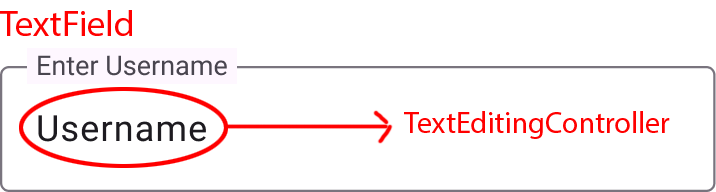
\includegraphics[width=0.5\linewidth, keepaspectratio]{Assets/Username_Field_verbose.png}}
	\caption{Rappresentazione grafica del TextField}
	\label{fig:textfield_verbose}
\end{figure}
\noindent

\subsubsection{Provider} \label{subsub:provider}
Provider \cite{provider} è una classe Flutter che gestisce la condivisione dei dati tra Widget. Questa classe permette di posizionarsi in modo globale all'interno dell'applicazione in modo che possa essere accessibile da chiunque e in qualunque punto dell'applicazione. Un aspetto importante è inoltre la sua capacità di agire come intermediario tra i Widget: quando un componente desidera apportare modifiche a qualcosa al di fuori del proprio scope, può richiedere al "Provider" di notificare direttamente l'elemento interessato affinché si "aggiorni". Per meglio comprendere questo concetto, esaminiamo il seguente esempio:
\begin{figure}[H]
	\centering
	\makebox[\textwidth] [c]{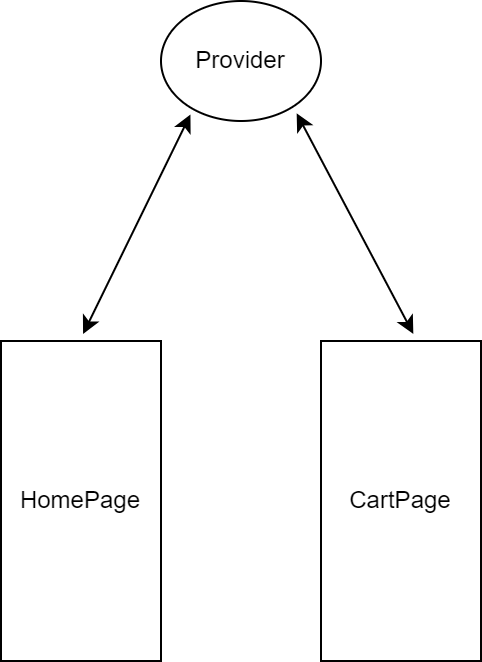
\includegraphics[width=0.5\linewidth, keepaspectratio]{Assets/diagram 1.png}}
	\caption{Rappresentazione grafica del Provider come intermediario}
	\label{fig:provider_example1}
\end{figure}
\noindent
Com'è facilmente intuibile, prendendo come esempio la pagina "Home" e del "Carrello", il Provider si comporta come intermediario tra le 2, essendo una classe a portata globale.\\
Immaginiamo ora che queste due pagine desiderino condividere una lista, specificamente l'elenco dei prodotti che l'utente ricerca e seleziona. Quando questo si trova nella pagina "Home" e aggiunge un elemento a questa lista, il "Provider" avvertirà la pagina del "Carrello" che è stato aggiunto un nuovo elemento. Di conseguenza, la pagina del "Carrello" si aggiornerà con i nuovi dati. Questa dinamica può essere illustrata nel seguente schema:
\begin{figure}[H]
	\centering
	\makebox[\textwidth] [c]{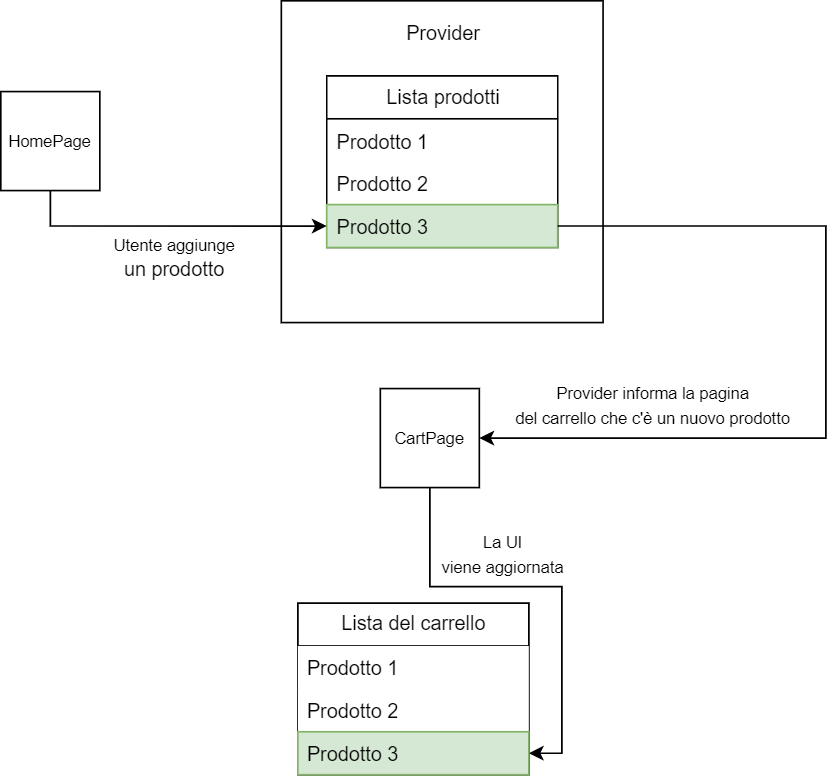
\includegraphics[width=1\linewidth, keepaspectratio]{Assets/diagram 2.png}}
	\caption{Condivisione dei dati e aggiornamento UI}
	\label{fig:provider_example2}
\end{figure}

\noindent
Tuttavia, questo Widget non è solo utile per condividere dati tra diverse pagine, ma anche tra componenti all'interno della stessa pagina. Dato che Flutter è fortemente orientato ai Widget, spesso accade che due di questi siano definiti in file separati, il che può rendere complicata la comunicazione tra componenti interni situati in Widget diversi. Prendiamo ad esempio la pagina del carrello, composta da due Widget: una lista e un testo che indica il totale dell'importo. Per farli comunicare efficacemente, essendo situati in due scope differenti, si può fare uso del "Provider". Quando l'utente modifica, ad esempio, la quantità di un prodotto, la lista imposta nel "Provider" il nuovo "importo totale" e il "Provider" si occuperà di notificare al "Widget testo" di aggiornarsi con il nuovo valore. Questa dinamica può essere chiaramente rappresentata attraverso il seguente schema:
\begin{figure}[H]
	\centering
	\makebox[\textwidth] [c]{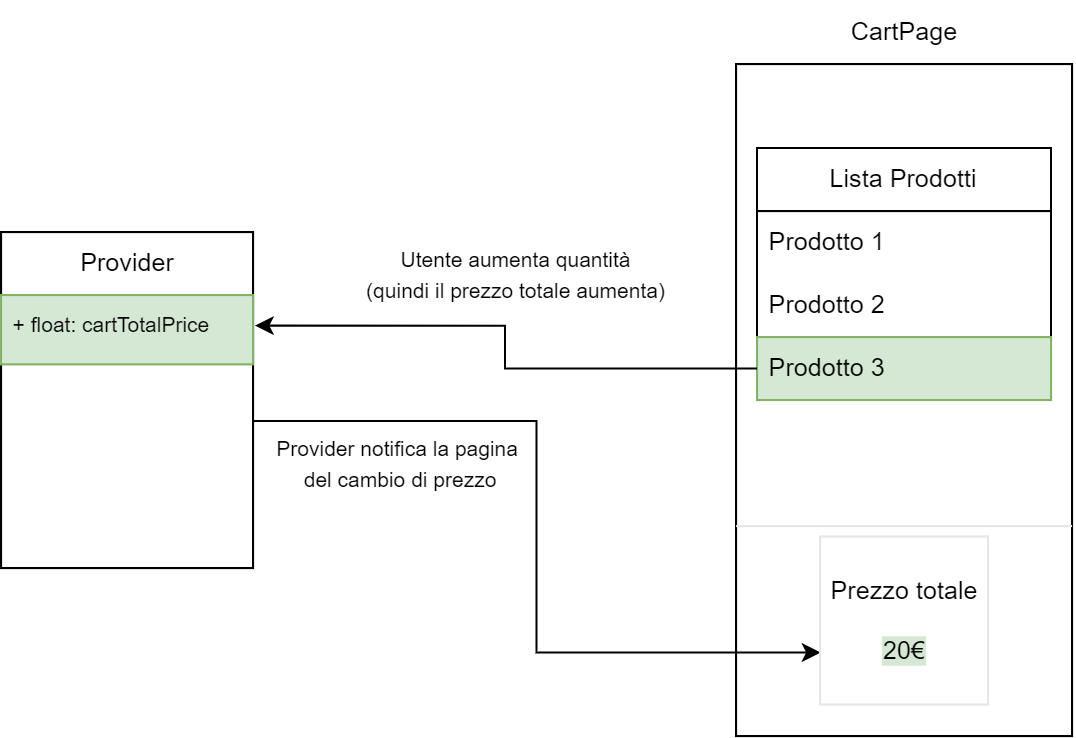
\includegraphics[width=1\linewidth, keepaspectratio]{Assets/diagram 3.png}}
	\caption{Condivisione dei dati tra componenti interni}
	\label{fig:provider_example3}
\end{figure}

\noindent

\paragraph{Selector}
Per consentire al "Provider" di individuare quale Widget deve essere aggiornato, è essenziale inserire il componente interessato dentro un "Selector" \cite{selector}. Questo Widget consente di specificare quale variabile del "Provider" deve essere monitorata. In tal modo, quando il "Provider" emette una notifica di cambiamento, il "Selector" verifica se l'aggiornamento riguarda la variabile monitorata e, in caso affermativo, aggiorna il componente con il nuovo valore.

\subsubsection{FutureBuilder} \label{subsub:futurebuilder}
Questo Widget è stato progettato per gestire le operazioni asincrone in modo semplice ed efficace, consentendo lo sviluppo di interfacce utente reattive e fluide. Il suo scopo principale è quello di semplificare l'integrazione dei dati asincroni, come il recupero di informazioni da Server o Database, all'interno dell'interfaccia utente. Il FutureBuilder \cite{future_builder} accetta un "future" come input, che rappresenta un'operazione (cioè una funzione) che potrebbe richiedere del tempo per essere completata. Durante l'attesa del completamento, il FutureBuilder è in grado di mostrare un'interfaccia temporanea, come un caricamento o una schermata con dati iniziali, in modo da non bloccare l'interfaccia durante il caricamento dei dati.

\subsubsection{FadeInImage} \label{subsub:fadeinimage}
FadeInImage \cite{fadeinimage} è un Widget Flutter la cui funzione principale è quella di sostituire gradualmente un'immagine di placeholder con un immagine finale, ottenuta da un URL. Il FadeInImage richiede due immagini come input: un'immagine di "placeholder" da visualizzare inizialmente, mentre l'immagine finale è in corso di caricamento, e quella effettiva che verrà mostrata una volta scaricata. Quando è finito lo scaricamento, il FadeInImage applicherà un effetto di dissolvenza graduale tra queste due immagini, creando un effetto visivo piacevole e delicato.

\section{Librerie impiegate}
\subsection{Javalin}
Javalin \cite{javalin} è un framework web scritto in linguaggio di programmazione Java, progettato per semplificare lo sviluppo di applicazioni web. Si concentra sulla semplicità e facilità d'uso, offrendo uno strato di astrazione per gestire le richieste HTTP e le risposte in modo pulito ed efficiente. Sebbene sia minimalista, Javalin offre ancora funzionalità essenziali come il routing delle richieste, la gestione dei parametri, il supporto per la creazione di endpoint RESTful e la gestione dei middleware.

\subsection{JWT} \label{sub:jwt}
JWT \cite{JWT_lib} è la libreria ufficiale che permette la creazione di token firmati mediante semplici metodi. Questa libreria è stata usata, per l appunto, per creare i token e verificarli una volta ricevuti dal Client.

\subsection{JUnit}
JUnit \cite{junit} è un framework di test unitari per il linguaggio di programmazione Java. Esso fornisce una struttura per scrivere, eseguire e organizzare test automatizzati per verificare il corretto funzionamento delle singole unità di codice, come metodi o classi, in isolamento dal resto dell'applicazione.
Il framework offre annotazioni, asserzioni e metodi di configurazione che semplificano il processo di scrittura e l'esecuzione dei test. Questa libreria è stata usata in quanto richiesta dal mio tutor aziendale.

\subsection{GSON}
GSON \cite{gson} è una libreria di Google che permette di convertire/serializzare un oggetto Java in testo JSON mediante dei semplici metodi ".toJson()" e ".fromJson()".

\subsection{SQLite}
SQLite \cite{sqlite} è una libreria che permette l'utilizzo di Database senza avere un vero e proprio DBMS. Di fatto, viene salvato tutto in file locali ed è possibile utilizzare il linguaggio SQL per gestire e manipolare le tabelle. Questa libreria consente quindi di avere un vero e proprio Database locale nel quale salvare i dati importanti in modo facile e veloce.

\subsection{Lottie}
Lottie \cite{lottie} è la libreria ufficiale sviluppata dall'azienda "Lottie" che permette di visualizzare le animazioni scaricate dal sito, in formato JSON, dentro ai Widget.

\paragraph{Material Dialog}
Material Dialog \cite{material_dialog} è la libreria che fa uso di Lottie per mostrare dei dialog animati comprensivi di titolo, descrizione e pulsanti a scelta.